\chapter{\MakeUppercase{Utilizando \LaTeX}}\label{sec:latex}

Este capítulo apresenta o uso básico de equações, figuras e tabelas no código da monografia, bem como o posicionamento das legendas, segundo as normas da UFLA. O LaTeX é um sistema de preparação de documentos que se destaca pela sua capacidade de criar documentos com alta qualidade tipográfica e estrutural. Sua força reside em uma série de elementos fundamentais que, combinados, permitem ao usuário ter controle granular sobre a aparência e a organização do conteúdo.


\section{O Básico Sobre Comandos \LaTeX}

Os \textbf{comandos} são a espinha dorsal do LaTeX. Eles são instruções que ditam como o texto e outros elementos devem ser processados e formatados. A maioria dos comandos começa com uma barra invertida (\verb|\|) e é seguida pelo nome do comando. Existem diferentes tipos de comandos.

\begin{alineas}
	\item \textbf{comandos sem argumentos:} são simples chamadas para uma ação. Exemplos incluem \verb|\maketitle| (para gerar o título do documento, se definido) ou \verb|\newpage| (para iniciar uma nova página);
	
	\item \textbf{comandos com argumentos obrigatórios:} esses comandos exigem que você forneça informações específicas entre chaves (\verb|{}|). Um exemplo clássico é:
	\begin{lstlisting}[language={[LaTeX]TeX}]
\section{Título da Seção}
	\end{lstlisting}
	Onde "Título da Seção" é o argumento que define o nome da seção;
		
	\item \textbf{comandos com argumentos opcionais:} além dos argumentos obrigatórios, alguns comandos podem aceitar \textbf{opções} entre colchetes (\verb|[]|). Essas opções modificam o comportamento padrão do comando. Por exemplo:
		\begin{lstlisting}[language={[LaTeX]TeX}]
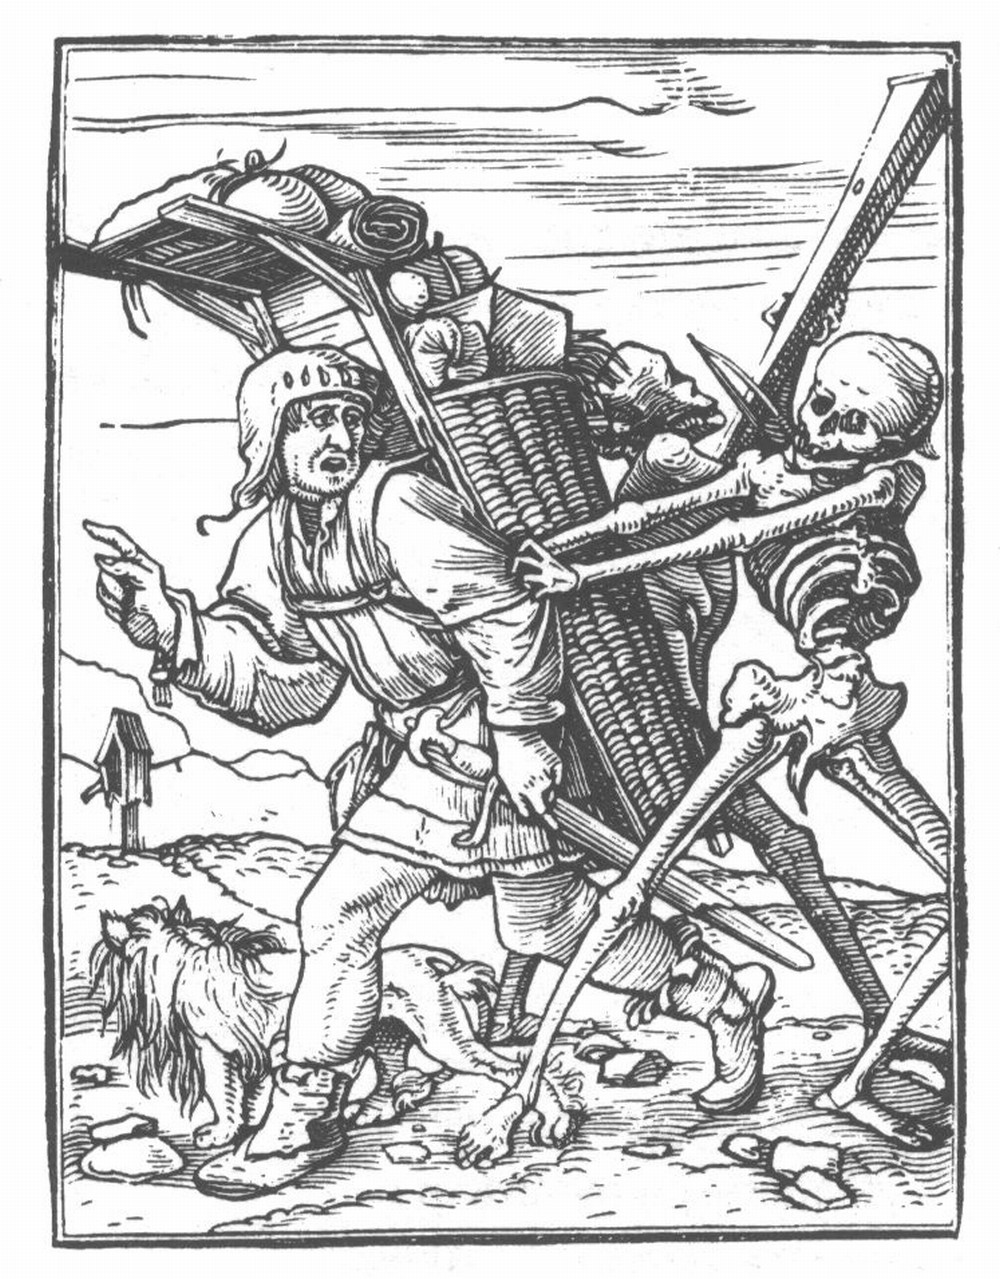
\includegraphics[scale=0.3]{imgs/exemplo}
		\end{lstlisting}
	O valor \verb|scale=0.3| é uma opção para definir que a imagem deve ter 30\% do seu tamanho original;
	
	\item \textbf{comentários:} além dos comandos, existem também os comentários, representados pelo sinal porcentagem (\texttt{\%}). Eles dizem para o interpretador do código que ignore todo o texto após o sinal. Em alguns casos (como quebras de linhas após abertura de colchetes), utiliza-se o sinal \texttt{\%} para que não haja espaços horizontais desnecessários.
\end{alineas}

\section{Adicionando arquivos no documento principal}

Em projetos \LaTeX, é comum ter um arquivo principal, onde se cria-se o preâmbulo (o que vem antes do \verb|\begin{document}|), estabelece-se a classe do documento, importa-se os pacotes e os configura. Para manter este arquivo o mais bem organizado e sucinto possível, recomenda-se que as seções, anexos e apêndices sejam colocados em arquivos externos próprios e importados para o arquivo principal utilizando os comandos \verb*|\include{arquivo}| ou \verb*|\input{arquivo}|. Esses comandos têm algumas importantes semelhanças e diferenças:

\begin{alineas}
	\item \textbf{semelhanças:} Ambos os comandos agem como um ``copia e cola'', adicionando o código dos arquivos externos ao arquivo principal sem a criação de nenhum ambiente especial. Dessa forma, caso não seja criado um ambiente especial manualmente, todas as configurações do arquivo principal são mantidas nos externos e todas as alterações feitas nos externos serão adicionadas ao ambiente principal. Além disso, o caminho usado nos arquivos externos é o mesmo do principal, por exemplo: se o arquivo principal está na pasta \textbf{\texttt{projeto}}, as imagens estão contidas na pasta \textbf{\texttt{projeto/imgs}} e um arquivo externo está em \textbf{\texttt{projeto/secoes}}, no arquivo externo as imagens serão acessadas em \textbf{\texttt{imgs}} e não em \textbf{\texttt{../imgs}};
	
	\item \textbf{diferenças:} esses comandos diferem, principalmente em como os conteúdos são adicionados:
	\begin{alineas}
		\item \textbf{\texttt{input}:} os códigos externos são adicionados ``como são'', ou seja, o comando funciona diretamente como um ``copia e cola'' automático e pode ser adicionado em qualquer lugar do código, até mesmo aninhados dentro dos arquivos externos;
		
		\item \textbf{\texttt{include}:} o comando \texttt{include} também insere códigos externos, mas os processa de maneira diferente. Ele sempre inicia uma nova página antes do conteúdo importado e não pode ser aninhado. Assim, é ideal que seja usado somente para elementos que comecem uma nova página, como capítulos de livros e seções primárias de trabalhos acadêmicos no formato da ABNT.
	\end{alineas}
\end{alineas}

\section{Comandos de Texto}

O \LaTeX\ oferece uma rica coleção de comandos dedicados à \textbf{formatação e estilização do texto}. Esses comandos permitem controlar a aparência do texto, como o estilo da fonte, o tamanho e a ênfase.
Aqui estão alguns dos comandos de texto mais frequentemente utilizados:

\begin{alineas}
	\item \textbf{ênfase e estilo da fonte:}
	\begin{alineas}
		\item \verb|\textbf{texto}|: produz texto em \textbf{negrito};
		\item \verb|\textit{texto}|: produz texto em \textit{itálico};
		\item \verb|\texttt{texto}|: produz texto em \texttt{monoespaçado} (fonte de máquina de escrever), útil para código ou nomes de arquivos;
		\item \verb|\textsf{texto}|: produz texto em \textsf{sans-serif} (sem serifa);
		\item \verb|\underline{texto}|: sublinha o \underline{texto};
		\item \verb|\emph{texto}|: aplica \emph{ênfase} ao texto. A forma como a ênfase é aplicada (itálico, negrito, etc.) pode depender do contexto e da classe do documento;
		\item \verb|\textsc{texto}|: gera texto em \textsc{SmallCaps}. Comum em nomes de algoritmos.
	\end{alineas}
	
	\item \textbf{tamanho da fonte:} o \LaTeX\  possui uma série de comandos para alterar o tamanho da fonte de forma relativa ao tamanho base do documento. É importante notar que estes comandos não aceitam argumentos e afetam todo o texto subsequente até que outro comando de tamanho seja utilizado, ou até o fim de um grupo delimitado por chaves:
	\begin{alineas}
		\item \verb|\tiny|: {\tiny texto muito pequeno;}
		\item \verb|\scriptsize|: {\scriptsize texto bem pequeno;}
		\item \verb|\footnotesize|: {\footnotesize texto pequeno;}
		\item \verb|\small|: {\small texto um pouco menor que o normal;}
		\item \verb|\normalsize|: {\normalsize tamanho de texto padrão (geralmente o padrão);}
		\item \verb|\large|: {\large texto grande;}
		\item \verb|\Large|: {\Large texto maior;}
		\item \verb|\LARGE|: {\LARGE texto ainda maior;}
		\item \verb|\huge|: {\huge texto enorme;}
		\item \verb|\Huge|: {\Huge texto realmente enorme.}
	\end{alineas}
	Para esse template, o comando mais importante é o \verb|\small|, que gera texto em 11pt, utilizado para notas, indicar a fonte de figuras e etc;
	
	\item \textbf{quebras de linha e espaçamento:}
	\begin{alineas}
		\item \verb|\\|: força uma quebra de linha;
		\item \verb|\newline|: também força uma quebra de linha, mas é mais robusto em alguns contextos;
		\item \verb|\linebreak|: sugere um ponto de quebra de linha, mas permite ao LaTeX ignorá-lo se não for ideal;
		\item \verb|\hspace{comprimento}|: insere um espaço horizontal com o comprimento especificado (ex: \verb|\hspace{1cm}|);
		\item \verb|\vspace{comprimento}|: insere um espaço vertical com o comprimento especificado (ex: \verb|\vspace{0.5cm}|).
	\end{alineas}
	
	\item \textbf{listas e tabulações simples (para texto corrido):} embora existam ambientes específicos para listas (\texttt{itemize}, \texttt{enumerate}) e tabelas (\texttt{tabular}), para alinhamentos simples em texto corrido, podem ser usados:
	\begin{alineas}
		\item \verb|\quad| e \verb|\qquad|: inserem espaços horizontais fixos maiores;
		\item \verb|\tabto{posição}|: para alinhar texto em uma posição específica, embora seja mais complexo e menos comum para iniciantes.
	\end{alineas}
\end{alineas}

O domínio desses comandos de texto permite um controle preciso sobre a apresentação visual do seu documento, garantindo que a mensagem seja transmitida com a clareza e o impacto desejados.





\section{Figuras} \label{sec:latexFiguras}

\begin{figure}[hbt!]
	\centering
	\caption{Uma Figura de Exemplo}\label{fig:exemplo} %legenda e referência
	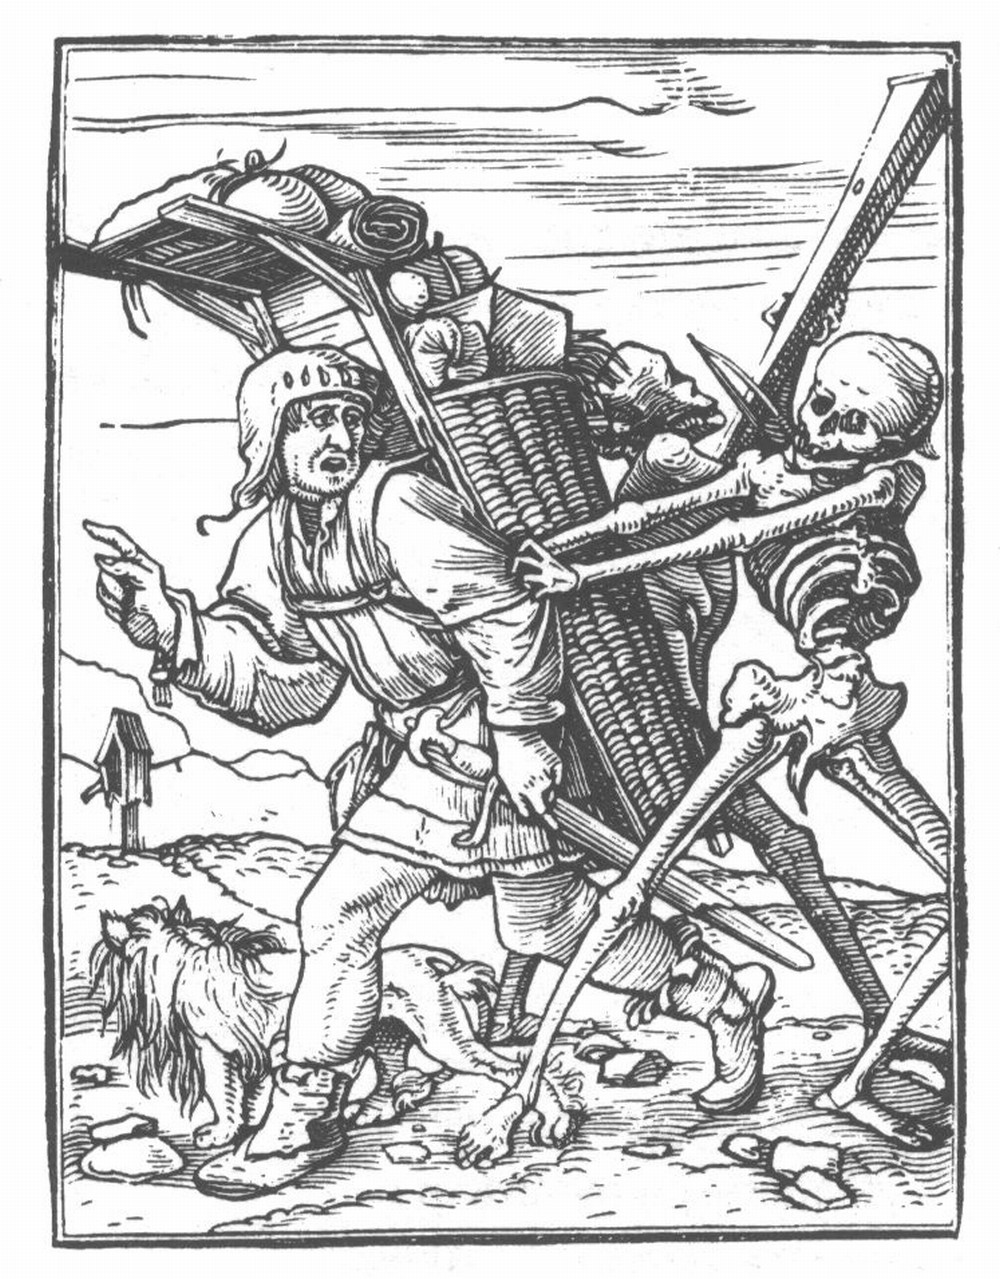
\includegraphics[scale=0.3]{imgs/exemplo}
	\fonte{fonte da figura (domínio público)} %Fonte da imagem
\end{figure}

A inclusão de \textbf{figuras} é um aspecto fundamental em muitos documentos, especialmente em trabalhos acadêmicos, relatórios técnicos e apresentações. A \autoref{fig:exemplo} é um exemplo de uma figura adicionada, O \LaTeX, em conjunto com o pacote \texttt{graphicx}, oferece um controle robusto sobre a inserção, posicionamento e legendagem de imagens:

\begin{alineas}
	\item \textbf{o ambiente} \texttt{figure}\textbf{:} figuras no LaTeX são geralmente inseridas dentro do ambiente \texttt{figure}. Este é um ambiente "flutuante", o que significa que o LaTeX pode mover a figura para uma posição ideal na página para evitar quebras de página embaraçosas e garantir uma boa legibilidade. Em um comando:
	\begin{lstlisting}[language={[LaTeX]TeX}]
\begin{figure}[posicionamento]
	% Conteúdo da figura aqui
\end{figure}
	\end{lstlisting}
	As opções de posicionamento entre colchetes (\texttt{[]}) sugerem ao LaTeX onde tentar posicionar a figura:
	\begin{alineas}
		\item \texttt{h} (here): tenta colocar a figura exatamente onde ela aparece no código;
		\item \texttt{t} (top): coloca a figura no topo da página;
		\item \texttt{b} (bottom): coloca a figura na parte inferior da página;
		\item \texttt{p} (page): coloca a figura em uma página separada dedicada a figuras e tabelas;
		\item \texttt{H} (here, force): força a figura a ficar exatamente onde ela é colocada no código (requer o pacote `float`). Use com cautela.
	\end{alineas}
	
	\item \textbf{o comando} \verb|\includegraphics{}|\textbf{:} este é o comando principal para inserir arquivos de imagem. Ele deve ser usado dentro do ambiente \texttt{figure}.
	\begin{lstlisting}[language={[LaTeX]TeX}]
\includegraphics[opcoes]{nome_do_arquivo}
	\end{lstlisting}
	As opções são especificadas entre colchetes (\texttt{[]}) e permitem controlar o tamanho e a rotação da imagem:
	\begin{alineas}
		\item \texttt{width=largura}: define a largura da imagem (ex: \texttt{width=0.8}\verb|\linewidth| para 80\% da largura da linha);
		\item \texttt{height=altura}: define a altura da imagem;
		\item \texttt{scale=fator}: redimensiona a imagem por um fator (ex: \texttt{scale=0.5} para metade do tamanho original);
		\item \texttt{angle=graus}: rotaciona a imagem pelos graus especificados.
	\end{alineas}
	Os formatos de imagem suportados dependem do compilador LaTeX que você está usando. Por exemplo: PDFLaTeX (o mais comum; usado pelo Overleaf) suporta PDF, PNG, JPG; LaTeX tradicional suporta EPS. Para gráficos e diagramas, formatos vetoriais, como PDF e EPS, são preferidos.
	
	\item \textbf{legendas e rótulos:}
	\begin{alineas}
		\item \verb|\caption{Texto da Legenda}|: adiciona um título à figura. É fundamental para descrever o conteúdo da imagem e garantir que ela seja incluída na lista de figuras;
		\item \verb|\label{chave_referencia}|: cria um rótulo único para a figura. Isso permite referenciá-la em qualquer parte do texto usando \verb|\ref{chave_referencia}| (que gerará o número da figura) ou \verb|\autoref{chave_referencia}| (que gerará "Figura X"). Por exemplo, podemos referir à imagem de exemplo como \autoref{fig:exemplo} e o texto resultante, em PDF, redirecionará para a figura em questão quando clicado.
	\end{alineas}
	
	\item \textbf{centralizando figuras:} é comum centralizar figuras na página para uma melhor apresentação. Isso pode ser feito usando o comando \verb|\centering| dentro do ambiente \texttt{figure}:
	\begin{lstlisting}[language={[LaTeX]TeX}]
\begin{figure}[!htb]
	\centering
	\caption{Uma Figura de Exemplo}\label{fig:exemplo} 
	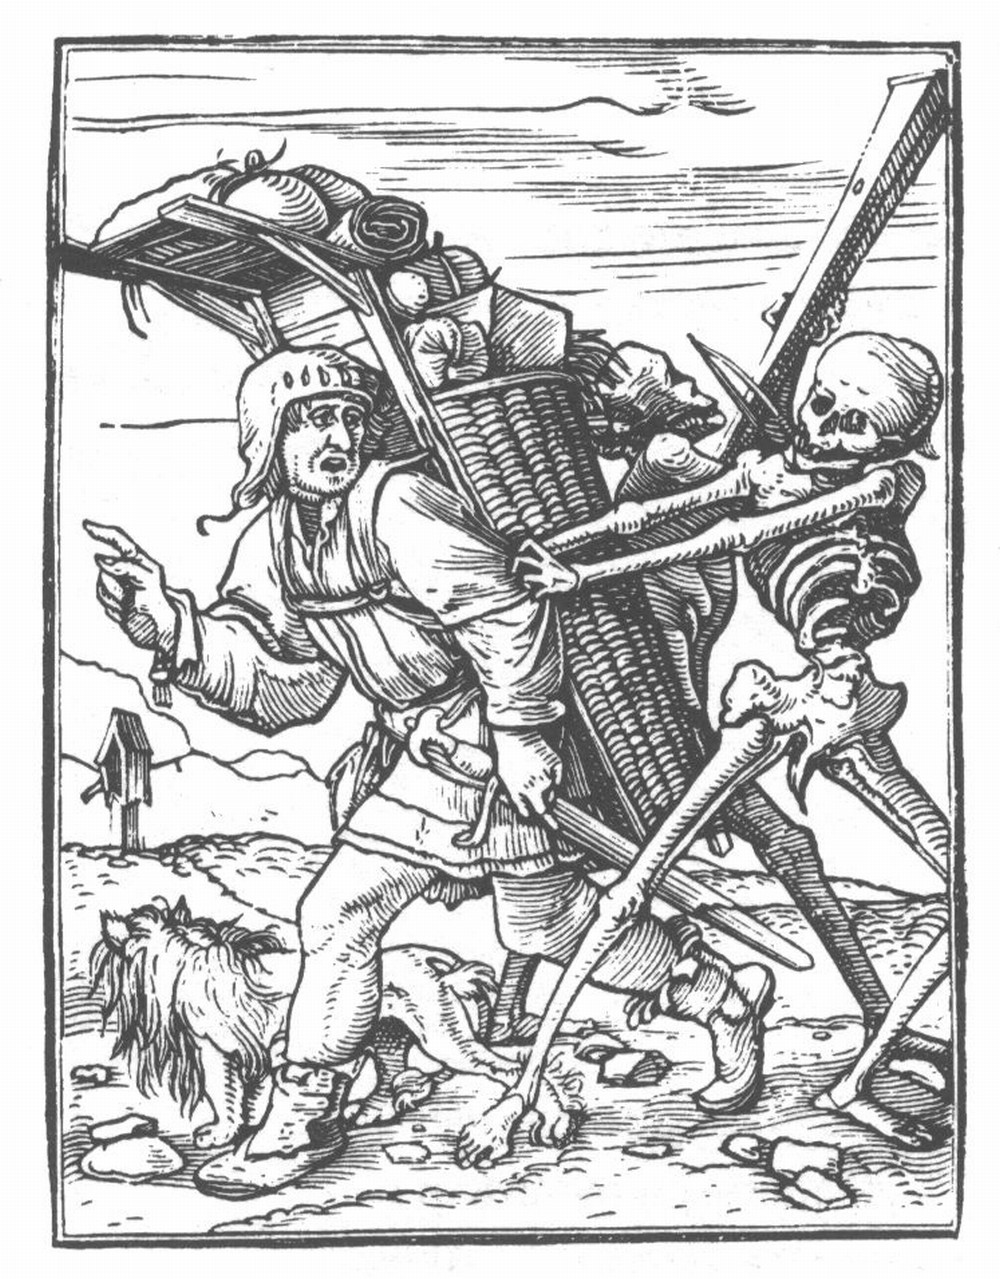
\includegraphics[scale=0.3]{imgs/exemplo}
	\fonte{fonte da figura (domínio público)} %Fonte da imagem
\end{figure}
	\end{lstlisting}
\end{alineas}

A correta utilização desses comandos e ambientes para figuras garante que suas ilustrações sejam incorporadas de forma profissional e acessível, complementando o conteúdo textual do seu documento.





\section{Ambientes Tabulares}

Tabelas são elementos cruciais para apresentar dados de forma organizada e legível em documentos científicos e acadêmicos. No \LaTeX, a criação de elementos tabulares é feita principalmente através do ambiente \texttt{tabular}, que oferece um controle preciso sobre a formatação e o alinhamento do conteúdo. A \autoref{tab:exemplo} é um exemplo.

\begin{table}[h!]
	\centering
	\caption{Exemplo de Tabela Flutuante com Fonte}\label{tab:exemplo}
	\begin{tabular}{l c r}
		\hline
		\linhadir{Cabeçalho 1} & \linhadir{Cabeçalho 2} & Cabeçalho 3 \\
		\hline
		Item 1 & Valor A & Nota X \\
		Item 2 & Valor B & Nota Y \\
		\hline
	\end{tabular}
	\vspace{.3cm}
	\fonte{original}
\end{table}

A estrutura fundamental de uma tabela em \LaTeX\  envolve o ambiente \texttt{tabular} e o uso de especificadores para definir o alinhamento das colunas e as linhas divisórias. Veja um exemplo simples:

\begin{lstlisting}[language={[LaTeX]TeX}]
\begin{tabular}{l c r}
  \hline
  \linhadir{Cabeçalho 1}& \linhadir{Cabeçalho 2}& Cabeçalho 3\\
  \hline
  Item 1& Valor A& Nota X\\
  Item 2& Valor B& Nota Y\\
  \hline
\end{tabular}
\end{lstlisting}
Nesse exemplo:

\begin{alineas}
	\item \texttt{\textbackslash begin\{tabular\}\{...\}} e \texttt{\textbackslash end\{tabular\}} delimitam o ambiente da tabela.
	\item os caracteres dentro das chaves \texttt{\{...\}} definem a formatação das colunas:
	\begin{alineas}
		\item \texttt{l} (left): alinha o conteúdo à esquerda;
		\item \texttt{c} (center): centraliza o conteúdo;
		\item \texttt{r} (right): alinha o conteúdo à direita;
		\item \texttt{|}: adiciona uma linha vertical entre as colunas.
	\end{alineas}
	\item \texttt{\&} é usado para separar o conteúdo de cada célula em uma linha;
	\item \texttt{\textbackslash\textbackslash} indica o fim de uma linha e o início da próxima;
	\item \texttt{\textbackslash hline} insere uma linha horizontal que abrange toda a largura da tabela.
\end{alineas}

\vspace{\baselineskip}

Para que sua tabela seja tratada como um ``float'' (flutuante), permitindo que o \LaTeX\  decida a melhor posição para ela no documento, e para que você possa adicionar uma legenda e referenciá-la, você deve encapsular o ambiente \texttt{tabular} dentro de um ambiente \texttt{table} ou \texttt{quadro}:

\begin{lstlisting}[language={[LaTeX]TeX}]
\begin{table}[h!]
	\centering
	\caption{Exemplo de Tabela Flutuante com Legenda}
	\label{tab:minhatabela}
	\begin{tabular}{l c r}
		\hline
		\linhadir{Cabeçalho 1}& \linhadir{Cabeçalho 2}& Cabeçalho 3\\
		\hline
		Item 1 & Valor A & Nota X \\
		Item 2 & Valor B & Nota Y \\
		\hline
	\end{tabular}
	\vspace{.3cm}
	\fonte{original}
\end{table}
\end{lstlisting}

Os comandos usados e suas explicacões são:
\begin{alineas}
	\item \texttt{\textbackslash begin\{table\}[h!]} e \texttt{\textbackslash end\{table\}}: delimitam o ambiente flutuante da tabela. As opções entre colchetes, como \texttt{[h!]}, sugerem ao \LaTeX\  a preferência de posicionamento (\texttt{h} para ``here'' - aqui, \texttt{!} para ``definitivamente aqui se possível''). Outras opções incluem \texttt{t} (top - topo da página), \texttt{b} (bottom - base da página) e \texttt{p} (page of floats - página dedicada a flutuantes);
	\item \texttt{\textbackslash centering}: centraliza a tabela na página;
	\item \texttt{\textbackslash caption\{...\}}: adiciona um título à tabela;
	\item \texttt{\textbackslash label\{...\}}: permite criar uma referência cruzada para a tabela usando\\ \texttt{\textbackslash ref\{tab:minhatabela\}} no texto, que será automaticamente atualizada com o número da tabela ou quadro, como \autoref{tab:exemplo};
	\item \texttt{\textbackslash fonte\{...\}}: usado para criar o texto da fonte. Deve vir após o \texttt{\textbackslash end\{tabular\}} e é ideal que tenha um espaço \texttt{\textbackslash vspace\{0.3cm\}} entre eles.
\end{alineas}

\subsection{Formatação Avançada}

\begin{table}[h!]
	\centering
	\caption{Exemplo de Tabela com recursos avançados}\label{tab:exemploAvan}
	% para alterar o espaçamento nos elementos tabulares
	\renewcommand{\arraystretch}{2.0} % altera espaçamento vertical (valor normal: 1.5)
	\setlength{\tabcolsep}{2ex} % altera espaçamento horizontal (valor normal: ~1ex)
	%
	% para tamanho horizontal fixo e quebra de linha na coluna
	%                 \/ 
	\begin{tabular}{m{2.5cm} c r}
		\hline
		\multirow{2}{2.5cm}{\bf Cabeçalho 2 linhas} & \multicolumn{2}{|c}{\bf Cabeçalho 2 colunas}\\
		\cline{2-3}
		% multicolumn abaixo necessário pelas linhas verticais (|c|)
		& \multicolumn{1}{|c|}{\bf Cabeçalho 2} & \bf Cabeçalho 3 \\
		\hline
		Item de valor um & Valor A & Nota X \\
		Item de valor dois & Valor B & Nota Y \\
		\hline
	\end{tabular}
	
	\vspace{.3cm}
	\fonte{original}
\end{table}

O \LaTeX\  oferece diversas opções avançadas para customizar suas tabelas, incluindo:

\begin{alineas}
	\item \textbf{linhas horizontais parciais:} use \texttt{\textbackslash cline\{i-j\}} para desenhar uma linha horizontal apenas das colunas \texttt{i} a \texttt{j};
	\item \textbf{células mescladas:} o pacote \texttt{multirow} permite mesclar células verticalmente\\ (\texttt{\textbackslash multirow\{num\_linhas\}\{largura\}\{conteúdo\}}) e o \texttt{multicolumn}\\ horizontalmente (\texttt{\textbackslash multicolumn\{num\_colunas\}\{alinhamento\}\{conteúdo\}});
	\item \textbf{espaçamento:} é possível ajustar o espaçamento entre linhas e colunas, além de usar pacotes como \texttt{booktabs} para criar tabelas com uma aparência mais profissional, focando em linhas mais finas e espaçamento aprimorado para melhorar a legibilidade.
\end{alineas}
A \autoref{tab:exemploAvan} é um exemplo de tabela que utiliza recursos avançados.

\vspace{\baselineskip}
Aprender a manipular tabelas no \LaTeX\  pode parecer complexo no início, mas o controle que ele oferece resulta em documentos com um visual extremamente polido e profissional, mantendo a consistência em todo o seu trabalho.


\section{Elementos Matemáticos}

Lidar com equações e símbolos complexos é uma das maiores vantagens do \LaTeX. Para inserir elementos matemáticos, você precisa estar em um \textbf{ambiente matemático}. Existem dois tipos principais de ambientes matemáticos:

\begin{alineas}
	\item \textbf{matemática em linha (inline math):} usada para equações curtas e símbolos que aparecem dentro do texto. Para entrar neste modo, você pode usar os delimitadores \verb|$$| ou \verb|\( ... \)|.\\
	Por exemplo: a frase ``a equação $E=mc^2$ é famosa. Ou, alternativamente, a equação \(E=mc^2\) é famosa'' pode ser escrita com:
	\begin{lstlisting}[language={[LaTeX]TeX}]
A equação $E=mc^2$ é famosa. Ou, alternativamente, a
equação \(E=mc^2\) é famosa. 
	\end{lstlisting}
	
	\item \textbf{matemática em exibição (display math):} usada para equações maiores que precisam de uma linha própria e que muitas vezes são numeradas. Para entrar neste modo, você pode usar os delimitadores \verb|$$| ou \verb|\[ ... \]|. A maneira mais comum e recomendada é usar o ambiente \texttt{equation} ou \texttt{align} (do pacote \texttt{amsmath}).\\
	Por Exemplo:
	\begin{lstlisting}[language={[LaTeX]TeX}]
$$
	\int_a^b f(x) \, dx = F(b) - F(a)
$$
	\end{lstlisting}
	Ou, preferencialmente:
	\begin{lstlisting}[language={[LaTeX]TeX}]
\begin{equation}
	\int_a^b f(x) \, dx = F(b) - F(a)
\end{equation}
	\end{lstlisting}
	O ambiente \texttt{equation} numera automaticamente a equação. Se você não quiser numerar, use \texttt{equation*}.
\end{alineas}



\subsection{Símbolos e Estruturas Comuns}

\LaTeX\ oferece uma vasta gama de símbolos e estruturas matemáticas. Aqui estão alguns dos mais utilizados:

\begin{alineas}
	\item \textbf{expoentes e subscritos:} use \verb|^| para expoentes e \verb|_| para subscritos. Se houver mais de um caractere, agrupe-os com chaves \verb|{}|:\\
	\textbf{Exemplo:} $x^2$, $a_{ij}$, $e^{i\pi}$.
	\begin{lstlisting}[language={[LaTeX]TeX}]
	$x^2$, $a_{ij}$, $e^{i\pi}$
	\end{lstlisting}
	
	
	\item \textbf{frações:} use \verb|\frac{numerador}{denominador}|:\\
	\textbf{Exemplo:} $\frac{1}{2}$, $\frac{x+y}{x-y}$.
	\begin{lstlisting}[language={[LaTeX]TeX}]
	$\frac{1}{2}$, $\frac{x+y}{x-y}$
	\end{lstlisting}
	
	\item \textbf{raízes:} use \verb|\sqrt{argumento}| para raiz quadrada e \verb|\sqrt[n]{argumento}| para a raiz n-ésima:\\
	\textbf{Exemplo:} $\sqrt{2}$, $\sqrt[3]{x^2+y^2}$.
	\begin{lstlisting}[language={[LaTeX]TeX}]
	$\sqrt{2}$, $\sqrt[3]{x^2+y^2}$
	\end{lstlisting}
	
	\item \textbf{somas e integrais:} use \verb|\sum| para somatórios e \verb|\int| para integrais. Os limites inferior e superior são adicionados com \verb|_| e \verb|^|, respectivamente:\\
	\textbf{Exemplo:} $\sum_{i=1}^n i^2$, $\int_a^b x^2 \, dx$.
	\begin{lstlisting}[language={[LaTeX]TeX}]
	$\sum_{i=1}^n i^2$, $\int_a^b x^2 \, dx$
	\end{lstlisting}
	
	\item \textbf{parênteses, colchetes e chaves ajustáveis:} para que os delimitadores se ajustem ao tamanho do conteúdo interno, use \verb|\left(| e \verb|\right)|, \verb|\left[| e \verb|\right]|, ou \verb|\left\{| e \verb|\right\}|:\\
	\textbf{Exemplo:} $\left(\frac{1}{2}\right)$, $\left[\sum_{i=1}^n x_i\right]$.
	\begin{lstlisting}[language={[LaTeX]TeX}]
	$\left(\frac{1}{2}\right)$,
		$\left[\sum_{i=1}^n x_i\right]$
	\end{lstlisting}
	
	\item \textbf{letras gregas:} basta digitar o nome da letra com uma barra invertida antes (a primeira letra maiúscula para a versão maiúscula):\\
	\textbf{Exemplo:} $\alpha$, $\beta$, $\Gamma$, $\Delta$.
	\begin{lstlisting}[language={[LaTeX]TeX}]
	$\alpha$, $\beta$, $\Gamma$, $\Delta$
	\end{lstlisting}
	
	\item \textbf{operadores matemáticos:} existem comandos para operadores como \verb|\sin|, \verb|\cos|, \verb|\log|, \verb|\lim|, etc:\\
	\textbf{Exemplo:} $\sin(x)$, $\log_2(x)$,$\lim_{x \to 0}\frac{\sin x}{x}$.
	\begin{lstlisting}[language={[LaTeX]TeX}]
	$\sin(x)$, $\log_2(x)$, 
		$\lim_{x \to 0}\frac{\sin x}{x}$
	\end{lstlisting}
	
\end{alineas}

\subsection{Pacote \texttt{amsmath}}

Para composições matemáticas mais avançadas e eficientes, é altamente recomendável incluir o pacote \texttt{amsmath} no preâmbulo do seu documento (\verb|\usepackage{amsmath}|). Ele oferece ambientes como \texttt{align} para alinhar múltiplas equações, \texttt{gather} para agrupar equações e muitos outros comandos úteis.

\subsection{Exemplo de Equação}
Abaixo, temos um exemplo de uma equação, utilizando o ambiente \texttt{equation}, que pode ser referenciada como \autoref{eq:exemplo}:


\begin{equation}
	\label{eq:exemplo}
	f(x) = \sum_{n=1}^{\infty} f^{(n)}(x)~~\frac{(x-a)^n}{n!}
\end{equation}


\section{Usando Referências}\label{sec:Refs}

Para gerenciar referências bibliográficas de forma eficiente no \LaTeX, pode-se utilizar o BibTeX. Ele permite que você mantenha sua bibliografia em um arquivo separado, tornando o processo de citação e a geração da lista de referências muito mais organizado e automatizado.

\subsection{Arquivo \texttt{.bib}}

Primeiro, é necessário um arquivo com a extensão \texttt{.bib} (por exemplo, \texttt{refbib.bib}). Neste arquivo, devem ser definidas todas as entradas bibliográficas usando um formato específico do BibTeX. É comum publicações online disponibilizarem entradas BibTeX prontas. O exemplo de uma entrada é:
\begin{lstlisting}[language={[LaTeX]TeX}]
@Book{Bookchin:1982, % identificador
	title     = {The Ecology of Freedom},
	author    = {Murray Bookchin},
	year      = 1982,
	publisher = {The Anarchist Library}
	url       = {https://theanarchistlibrary.org/library/murray-bookchin-the-ecology-of-freedom}
}
\end{lstlisting}
Existem diversos tipos de entrada (como \texttt{@book}, \texttt{@inproceedings}, \texttt{@misc}) e campos obrigatórios/opcionais para cada um.

\subsection{Citando no Texto}
Para citar uma referência em seu texto, basta usar o comando \verb|\cite{chave}|, onde chave é o identificador único que você definiu no seu arquivo \texttt{.bib}, e o sistema já faz todo o trabalho da formatação e adição na lista de referências.\par
Por exemplo, ``Exemplo da citação com cite: \cite{Bookchin:1982}.'' tem código:
\begin{lstlisting}[language={[LaTeX]TeX}]
Exemplo da citação com cite: \cite{Bookchin:1982}.
\end{lstlisting}

\subsection{Gerando Lista de Referências}
A lista de referências será gerada automaticamente no local onde você inserir o comando \verb|\bibliography{nomedoarquivo}|. Com \texttt{nomedoarquivo} sendo o nome do seu arquivo \texttt{.bib} (sem a extensão). As referências podem assumir diferentes estilos que podem ser alterados com o comando \verb|\bibliographystyle{estilo}|, com o estilo \texttt{plain}, por exemplo, gerando referências simples e enumeradas.